\chapter{Background}
\label{cha:Background}

\section{Deep learning}

\begin{definition}
  An \textit{Artificial Neural Network (ANN)} \autocite{oshea2015introductionconvolutionalneuralnetworks} \autocite{sharma2017activation} is a computational model inspired by the structure and function of biological neural networks. It consists of interconnected artificial neurons (or nodes), which collectively process input data and learn patterns through training.

  In the case of Feedforward Neural Networks (FNNs), neurons are organized into layers, with each neuron in one layer connected to every neuron in the subsequent layer via directed connections. These connections are associated with trainable parameters called weights. Other neural architectures, such as Restricted Boltzmann Machines (RBMs) and Recurrent Neural Networks (RNNs), use different strategies for grouping and connecting neurons to capture specific data structures or temporal dependencies.

  Each neuron in the network also possesses a bias term—another learnable parameter—used to adjust the activation threshold. The output of a neuron is computed as a function of the weighted sum of its inputs and its bias, passed through a non-linear activation function. During training, both weights and biases are updated to minimize the network’s prediction error and improve its performance.
\end{definition}

\begin{definition}
  An \textit{Activation Function} \autocite{sharma2017activation} is a mathematical function used in artificial neural networks to determine the output of a neuron based on its input, associated weights, and bias. Given a neuron with inputs \(x\), weights \(w\), and bias \(b\), the neuron computes a linear combination \(z = w^\top x + b\). The activation function is then applied to this linear output, producing the final output of the neuron. Activation functions introduce non-linearity into the network, enabling it to learn complex patterns and approximate arbitrary functions. Common activation functions include the Sigmoid, Hyperbolic Tangent (Tanh), and Rectified Linear Unit (ReLU).
\end{definition}

An activation function is typically expected to exhibit two key mathematical properties:
\begin{enumerate}
  \item \textbf{Nonlinearity} \autocite{augustine2024surveyuniversalapproximationtheorems}: To satisfy the conditions of the Universal Approximation Theorem and enable the network to model complex, non-linear relationships, activation functions must introduce nonlinearity into the system. Using a nonlinear activation function in hidden layers is essential for learning intricate patterns in the data, but linear functions are also sometimes used, e.g. in the output layer of neural networks.
  \item \textbf{Differentiability} \autocite{sharma2017activation}: The activation function should ideally be differentiable across its entire domain to allow the computation of gradients during backpropagation. This is necessary for calculating loss gradients with respect to the network’s weights, enabling optimization techniques like Gradient Descent. However, it is not strictly necessary for the function to be continuously differentiable. For instance, the Rectified Linear Unit (ReLU) is not differentiable at zero, yet it is widely used—particularly in combination with convolutional layers—due to its empirical effectiveness and computational efficiency.
\end{enumerate}

\begin{definition}
  \textit{Deep supervised learning} \autocite{alzubaidi2021review} \autocite{cun2015deeplearning} \autocite{oshea2015introductionconvolutionalneuralnetworks} is a machine learning approach that relies on labeled data to train deep neural networks. Let \(D_t\), denote the training dataset, where each example \((x_t, y_t) \in D_t\) consists of an input datapoint \(x_t\) and its corresponding output label \(y_t\). A function \(f\), typically represented by an artificial neural network (ANN), is learned to map inputs to outputs. The discrepancy between the predicted output \(f(x_t)\) and the true output \(y_t\) is quantified using a loss function \(\gamma\), yielding a loss value \(\gamma(y_t, f(x_t))\). Optimization techniques such as Gradient Descent are then used to iteratively update the network’s parameters in order to minimize the loss, thereby improving the model’s accuracy in approximating the target function.
\end{definition}

\section{Convolutional Neural Networks}

Convolutional Neural Networks (CNNs) are among the most widely used and powerful tools in the field of Computer Vision. They excel at tasks such as image classification, dimensionality reduction, and other operations involving high-dimensional data. One of their key advantages is the ability to efficiently extract meaningful features from images without the need to store vast numbers of parameters, making them highly effective for analyzing complex, multidimensional data. While CNNs are primarily designed for processing two-dimensional inputs, they can also be adapted for one-dimensional \autocite{8126078} or three-dimensional \autocite{9786658} data, enabling their use in applications like sequence prediction and volumetric data classification.

\begin{definition}
  A \textit{kernel} \autocite{alzubaidi2021review}, also known as filter, is a small matrix of learnable weights $K \in \mathbb{R}^{m \times n}$ (or a higher-dimensional tensor, depending on the input) used in the convolutional and pooling layers of a Convolutional Neural Network (CNN). In convolutional layers it performs the convolution operation by sliding across the input $X$, computing a dot product at each position:
  \[(X * K)(i, j) = \sum_{u=0}^{m-1} \sum_{v=0}^{n-1} X(i+u, j+v) \cdot K(u, v) \]
  This operation produces a feature map that highlights spatial patterns such as edges or textures. The kernel weights are optimized during training.
\end{definition}

\begin{definition}
  A \textit{convolutional operation} \autocite{alzubaidi2021review} is a process in which a kernel slides through the input image horizontally and vertically and dot product between kernel and input is calculated for each sliding point. The sliding and calculation of the dot product between matrices is performed until no further sliding is possible. The sliding can be performed by visiting every pixel in each direction, but kernel can also slide skipping one or multiple pixels, depending on the stride size of the layer. The grid of scalar values that appear after performing convolutional operation is usually called a feature map. An example of convolutional operation is shown in figure \ref{fig:convolution-diagram}.
\end{definition}

\begin{figure}[htbp]
  \centering
  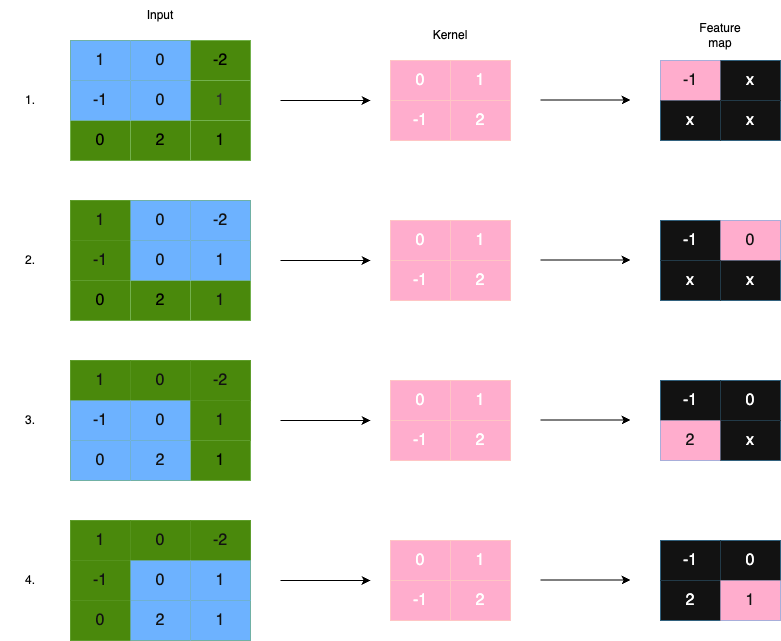
\includegraphics[width=0.8\textwidth]{Images/convolutional_operation.png}
  \caption{Illustration of the convolutional operation using a kernel on 2D input data.}
  \label{fig:convolution-diagram}
\end{figure}

\begin{definition}
  A \textit{Convolutional Neural Network (CNN)} \autocite{oshea2015introductionconvolutionalneuralnetworks} \autocite{jmse9040397} \autocite{LIU201711} is a discriminative deep learning model whose architecture is inspired by the hierarchical organization of the visual cortex in animals. CNNs are particularly effective in tasks involving image and spatial data processing due to their ability to capture local patterns and spatial hierarchies.

  The core components of a CNN are \textbf{convolutional layers} and \textbf{sub-sampling (pooling) layers}.

  \textbf{Convolutional layers} apply a set of learnable kernels (filters), each with its own weights, which slide over the input matrix to perform convolution operations. These layers extract local features by emphasizing patterns such as edges, textures, or more complex structures as the network deepens. They also preserve the spatial relationship between features, allowing the network to learn spatial hierarchies.

  \textbf{Sub-sampling layers}, also known as pooling layers, are used to progressively reduce the spatial dimensions of the feature maps. This helps decrease the computational complexity, control overfitting, and enhance the model’s invariance to small translations in the input. Common pooling operations include max pooling and average pooling, where the most prominent or average feature within a local region is retained. It's generally advised to use kernel size of 3 or less in pooling layers, due to their destructive nature and high chance of losing meaningful features.
\end{definition}

The concept of CNNs was inspired by Time-Delay Neural Networks, where weights are shared through time dimension. In CNNs weights are compacted into it's kernels. This architectural property vastly reduces the number of parameters and complexity of the network compared to Fully Connected Networks. CNNs are valued for their ability to learn to identify features without human interaction and for their empirically proven performance in processing multidimensional data with grid-like topology, like images and videos.